\documentclass[UTF8]{ctexart}
\usepackage{graphicx}
\usepackage{amsmath}
\usepackage{cite}
\usepackage{booktabs}
\usepackage[a4paper,left=2.5cm,right=2.5cm,top=3cm,bottom=3cm]{geometry}
\title{实验报告}
\author{禤科材 PB20030874 20级14系}
\date{\today}
\bibliographystyle{plain}

\begin{document}
    \maketitle
    \section{实验目的}
    测量合肥地区重力加速度

    \section{实验原理}
    根据牛顿运动定律,自由落体的运动方程为:\cite{jiangyi}
    \begin{equation}
        h=\frac{1}{2}gt^2
    \end{equation}
    本实验采用双光电门法测$t$.通过固定通过光电门$1$使得$\nu_0$保持不变,小球通过光电门$1$与光电门$2$
    的高度差为$h$,时间差为$t$ ,通过改变光电门$2$的位置,则能测量到一系列$h_i-t_i$的数据

    将自由落体公式修正为:\cite{jiangyi}
    \begin{equation}
        \frac{h}{t}=\nu_0+\frac 12 gt
    \end{equation}
    以$\frac{h_i}{t_i}-t_i$作图,预计应当是线性关系,利用线性拟合最小二乘法求出重力加速度$g$

    \section{实验步骤}
    以重力线为基准调节架台,使其与地面垂直,棉线通过光电门中心位置

    打开电磁毫秒计,将小球吸附在电磁铁上

    关闭电磁铁,释放小球,同时开始计时,记录数据

    调节光电门$2$的位置,重复试验6次


    \section{自由落体法测量重力加速度实验数据表}

    
    \begin{center}
        
        \begin{tabular}{lllllll}
            $t_1(ms)$       & 135.7 & 136.2 & 135.8 & 136.1 & 135.9 & 135.5 \\
            $t_2(ms)$       & 243.2 & 282.6 & 316.2 & 347.4 & 375.3 & 401.5 \\
            $t_2-t_1(ms)$   & 107.5 & 146.4 & 180.4 & 211.3 & 239.4 & 266.0 \\
            $h(cm)$         & 20.00 & 30.00 & 40.00 & 50.00 & 60.00 & 70.00 \\
            \hline
        \end{tabular}
        
    实验人:禤科材

    实验仪器:自由落体仪,接收器,卷尺

    实验日期:2021.4.2

    \end{center}
    
    
    \section{数据处理}
    使用scidavis软件\footnote{IOS系统的ORIGIN替代品}作图如下:
    \begin{figure}[ht]
        \centering 
        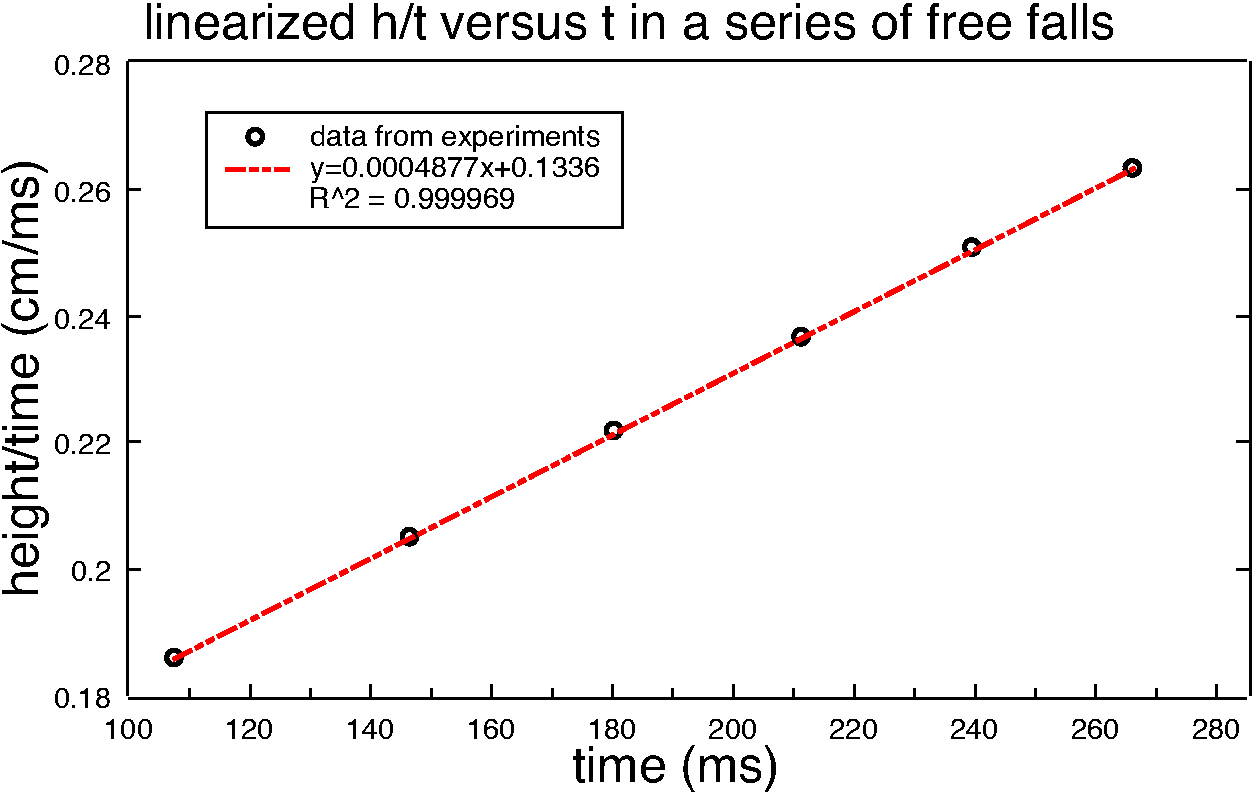
\includegraphics[width=13cm]{linearized.pdf}
    \end{figure}

    \emph{斜率$k$的标准差:}\cite{daolun}
    \begin{equation}
        \sigma_k =k\sqrt{(\frac{1}{R^2}-1)/(n-2)}=0.0004877\sqrt{(\frac{1}{0.999969}-1)/(6-2)} =0.0000013
    \end{equation}

    \emph{斜率$k$展伸不确定度:}\cite{daolun}
    \begin{equation}
        U_{0.95}=t_p·\sigma_k=2.78·0.0000013=0.000004=0.04m·s^{-2}
    \end{equation}

    \emph{截距$b$标准差:}\cite{daolun}
    \begin{equation}
        \sigma_b=\sqrt{\overline{{x^2}}}·\sigma_k=\sqrt{\frac{107.5^2+146.4^2+180.4^2+211.3^2+239.4^2+266.0^2}{6}}·0.0000013=0、00027
    \end{equation}

    \emph{截距$b$展伸不确定度:}\cite{daolun}
    \begin{equation}
        U_{0.95}=t_{0.95}·\sigma_b=2.78·0.00027=0.00075cm·s^{-1}
    \end{equation}

    根据公式$\frac{h}{t}=\nu_0+gt$,计算知$g=2·4.877=9.754m·s^{-2}$


    \emph{最终结果:}
    \begin{equation}
        g=9.75±0.04m·s^{-2}
    \end{equation}

    由计算可知,$\frac{\varDelta g}{g}$<0.01,在设计精度内
    \section{误差分析}
    根据合肥重力加速度标准值为9.7947$m·s^{-2}$可知所测真值偏小,但实际值落在不确定度范围内。
    经分析,有以下几点原因:

    1.组成横轴的数据$t_1$方差较大,导致在计算过程中斜率的标准差增加,不确定度增大

    2.测量次数仅有6次,带入的$t_{0.95}=2.78$太大,再一次扩大不确定度,导致测量精确度降低

    3.测量真值偏小大约0.04,应当是由于光电门$1$设置过于靠近电磁铁,导致小球进入光电门后电磁铁还未完全消磁,处于磁铁引力范围内

    \section{提出改进}
    1.加高立柱,增加光电门$1$与电磁铁的距离,减小电磁力的影响

    2.增大数据密集度,在$1m$内尽量测量14-16个值,降低$t_p$

    3.改良电磁铁,使用消磁快的材料

    \section{思考题}
    1.因为$h=\frac{1}{2}gt^2$当且仅当初速度等于0的时候才成立,然而无论是实验者还是实验仪器,都无法测量释放的准确时间

    2.光电门1应当适当远离电磁铁,防止不完全消磁影响实验;光电门2应在光电门1正下方,且要尽量多的选取测量点,保证实验精确度

    3.将光电门2固定于待测位置,改变光电门1的高度,多次测量,利用最小二乘法反向线性拟合,截距即对应光电门2处的速度

    4.将光电门拆下,安装在水平木板上。取已知质量的小车,将小车通过轻绳与托盘连接,轻绳跨过桌边上的固定小滑轮。调节木板倾斜角度,直至小车匀速滑动。向托盘中加入已知质量的砝码,释放小车,记录小车上的遮光片通过光电门1、2的间隔。改变砝码质量、个数,重复试验,即可得到砝码质量与小车加速度的关系,由此测量重力加速度

    \nocite{jiaocheng}
    \nocite{shiyan}
    
    \bibliography{math}
\end{document}